\chapter{Early flood warning tool}
\label{chp:flood_warning_system}

An \textit{early flood warning tool} in an essential component of an \textit{early flood warning system}.
An early flood warning system has to be understood as an integrated system of tools and plans to detect and respond to flood emergencies \autocite{icimod_early_2018}.
This can be managed by the community themselves and if designed, implemented and operated correctly can make the difference between tragedy and survival.

Such systems have already been installed in various endangered regions in the world.
After the major flooding of July 2014, the city of Altstätten in the canton of St. Gallen made the decision to install one.
The system installed uses cameras, sensors and level meters to gather data and information about the current situation \autocite{st._galler_tageblatt_altstatten_2017}.
When the value of certain parameters exceed the given threshold, a dangerous situation is recognized and the alarm signal is sent.

Three years after the installation of the system an alarm rings in the middle of the night.
Firemen go immediately into action in order to install temporary measures to fight against the water.
A couple of hours later the torrent overflows at several points and the city gets flooded.
Damages are less severe than last time, especially thanks to the temporary measures installed, but possibly they could have been reduced even more.

Crucial in order to limit the damages is the intervention time before the actual flooding occurs.
The earlier the dangerous situation can be detected the more time is available to the population and authorities to get ready and set up different types of temporary mitigation measures.
Systems based on sensors monitoring the evolution of the current situation in the upper part of the catchment are quite reliable but do not allow for long anticipation time. 

Numerical simulations can be run with meteorological forcast data and approximate soil saturation conditions in order to obtain early predictions of the event outcome.
However, the big advantage of predicting with that much anticipation is partially lost due to the duration of such simulations.
Accurate meteorological forcasts are available only few hours before the event.
If the model require several hours to run, which is often the case to obtain accurate predictions for catchments of this extent, then the advantage of being able to run it in advance is cancelled.

A possible solution to this problem is the developement of an \emph{ad hoc surrogate model} exploiting the catchment specific behaviour.


\section{Methodology}

In order to run the simulations necessary for building the emulator, a synthetic topography was produced.
The synthetic topography, in comparison with a real one, 

Bla bla bla bla \autocite{octave_community_gnu_2018}.

\begin{figure}[htpb]
  \centering
  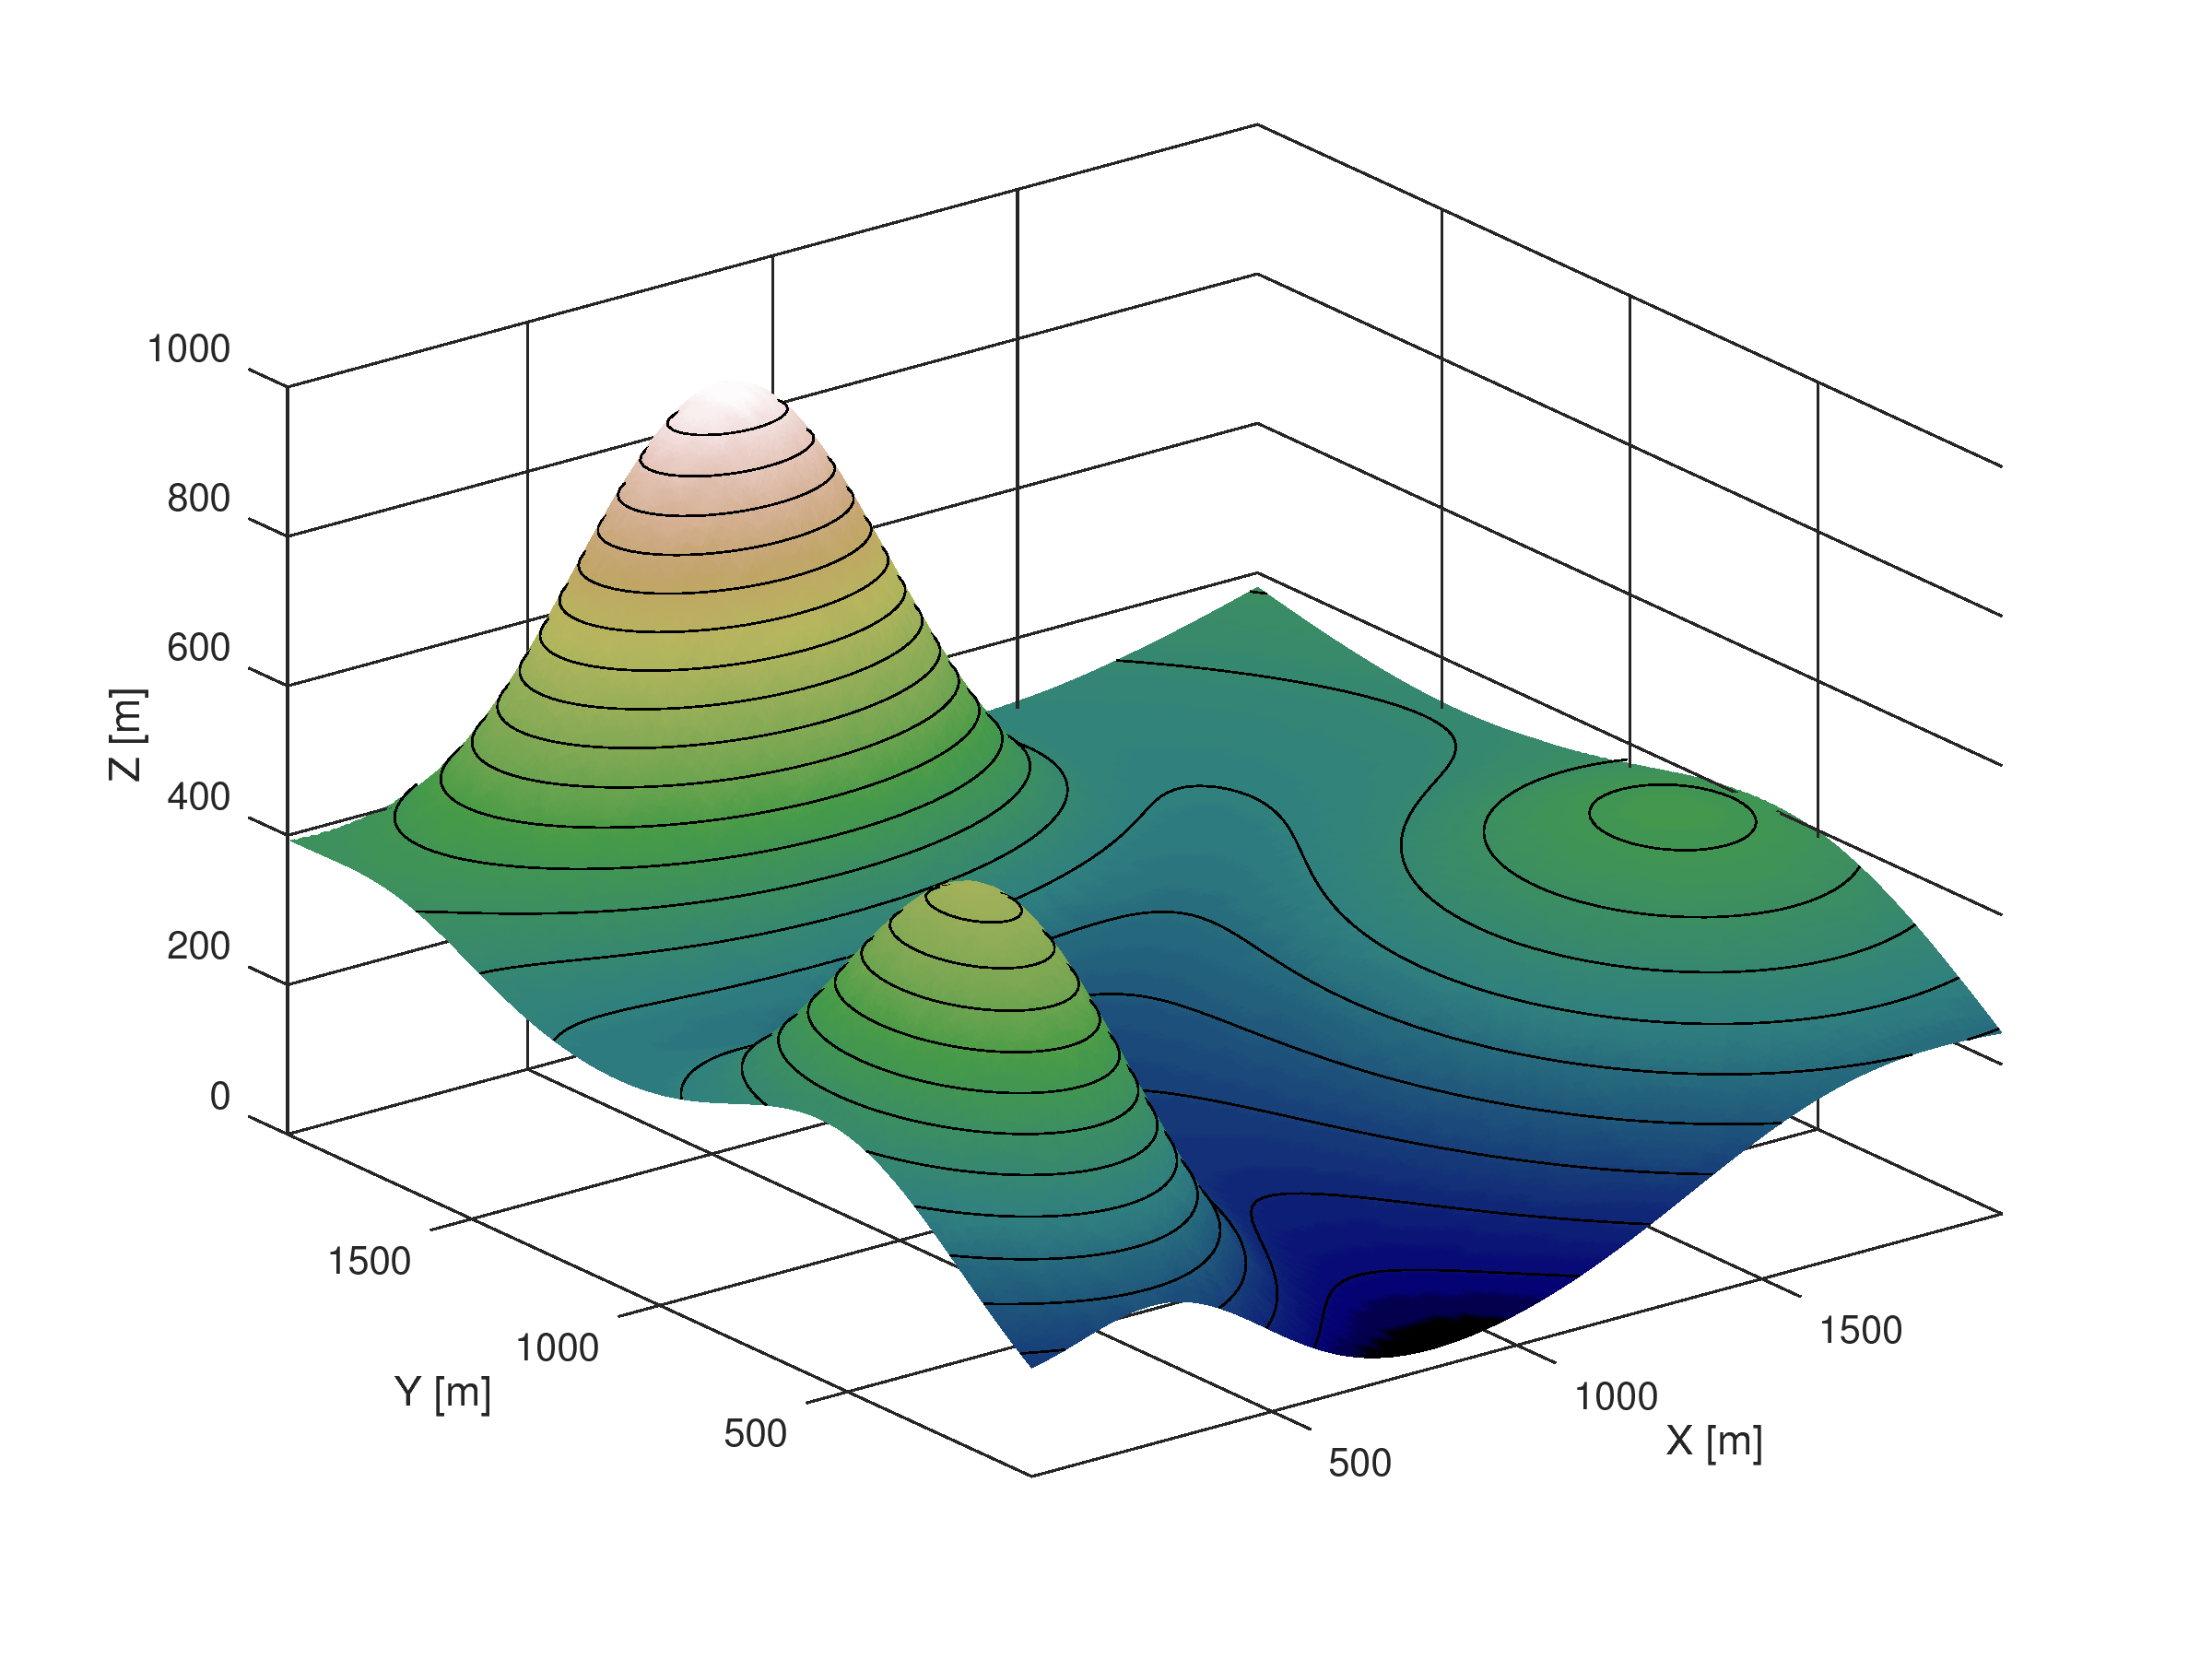
\includegraphics[width=0.7\textwidth]{../../../img/topography.png}
  \caption{Synthetic topography composed of three gaussian bumps on a sloping plane. A parabola centered on the middle axis of the plane was added to favour concentration of the flow towards the center.}
  \label{fig:topography}
\end{figure}

\section{Results}

